% $Id: WebServices_desc.tex,v 1.8 2012/01/06 20:19:24 svasquez Exp $
%
% Earth System Modeling Framework
% Copyright 2002-2013, University Corporation for Atmospheric Research, 
% Massachusetts Institute of Technology, Geophysical Fluid Dynamics 
% Laboratory, University of Michigan, National Centers for Environmental 
% Prediction, Los Alamos National Laboratory, Argonne National Laboratory, 
% NASA Goddard Space Flight Center.
% Licensed under the University of Illinois-NCSA License.

%\subsection{Description}

The goal of the ESMF Web Services is to provide the tools to allow ESMF Users to make 
their Components available via a web service.  The first step is to make the Component 
a service, and then make it accessible via the Web.  

\begin{center}
\begin{figure}
\caption{The diagram describes the ESMF Web Services software architecture. The architecture
defines a multi-tiered set of applications that provide a flexible approach for accessing
model components.}
\label{fig:webservices_fig}
\scalebox{0.5}{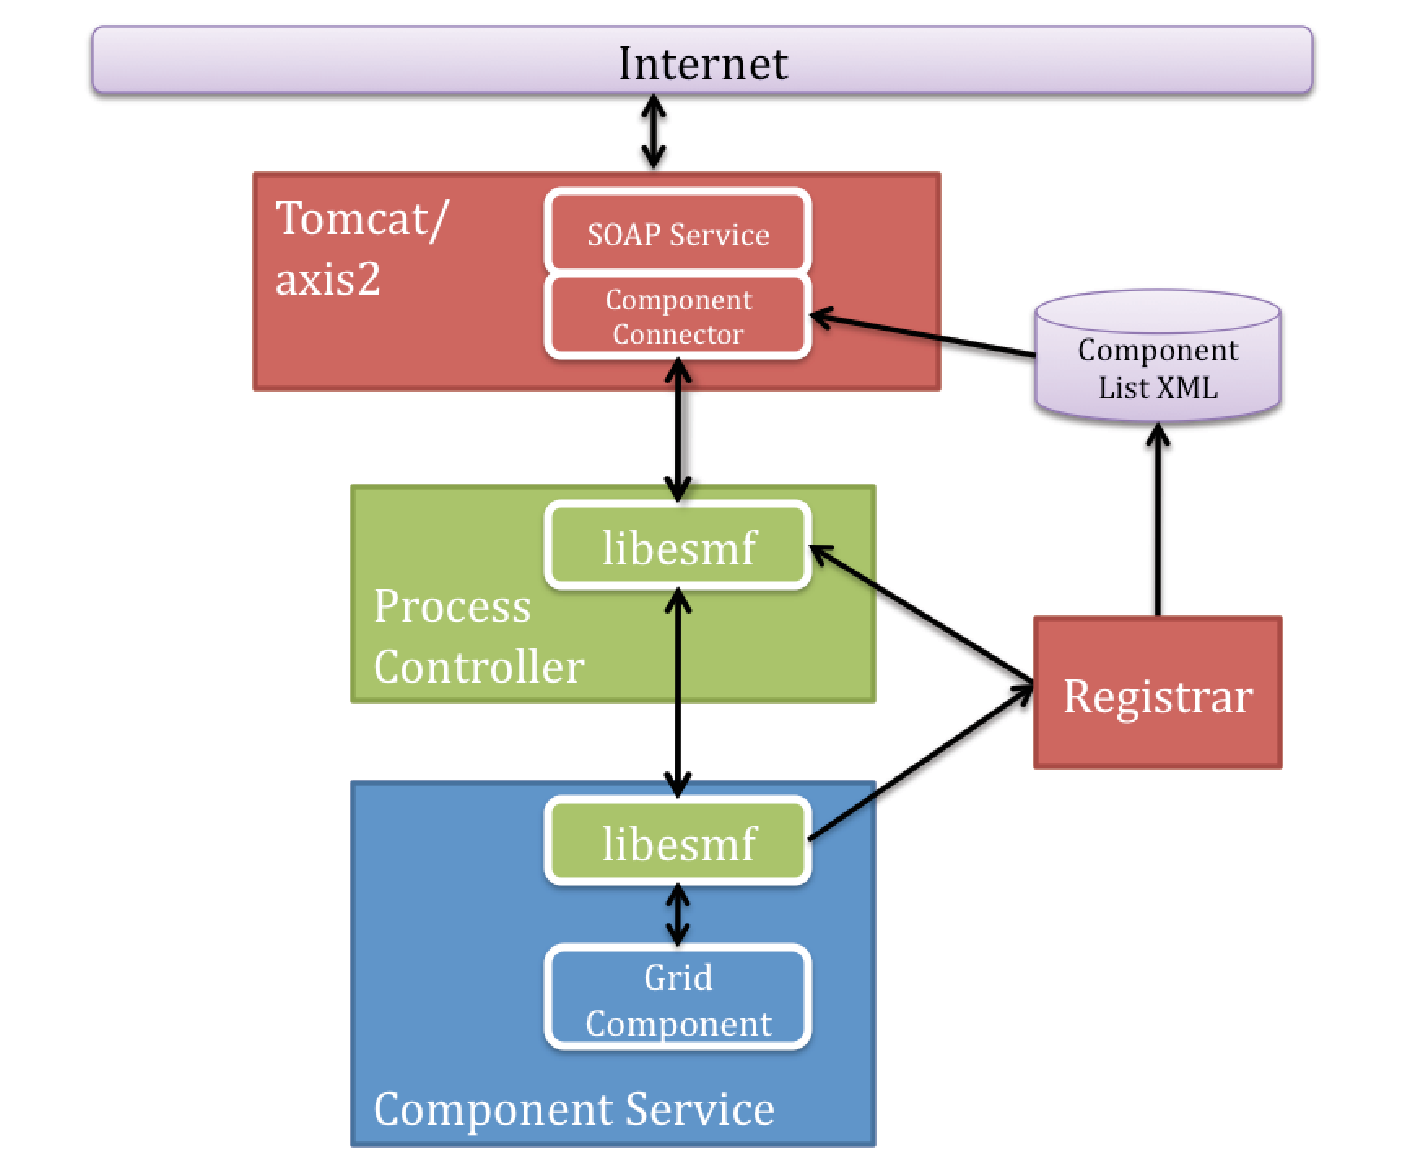
\includegraphics{webservices}}
\end{figure}
\end{center}

At the heart of this architecture is the Component Service; this is the 
application that does the model work.  The ESMF Web Services part provides a way to make 
the model accessible via a network API (Application Programming Interface). ESMF provides 
the tools to turn a model component into a service as well as the tools to access the 
service from the network. 

The Process Controller is a stand-alone application that provides a control mechanism between 
the end user and the Component Service.  The Process Controller is responsible for managing 
client information as well as restricting client access to a Component Service.  
(The role of the Process Controller is expected to expand in the future.)

The tomcat/axis2 application provides the access via the Web using standard SOAP 
protocols. Part of this application includes the SOAP interface definition 
(using a WSDL file) as well as some java code that provides the access to the Process 
Controller application.

Finally, the Registrar maintains a list of Component Services that are currently 
available;  Component Services register themselves with the Registrar when they 
startup, and unregister themselves when they shutdown.  The list of available services 
is maintained in an XML file and is accessible from the Registrar using its network API.

\subsubsection{Creating a Service around a Component}
\subsubsection{Code Modifications}
One of the goals in providing the tools to make Components into services was to make 
the process as simple and easy as possible.  Any model component that has been 
implemented using the ESMF Component Framework can easily be turned into a 
Component Services with just a minor change to the Application 
driver code.  (For details on the ESMF Framework, see the ESMF Developers Documentation.)

The primary function in ESMF Web Services is the ESMF\_WebServicesLoop routine.  This 
function registers the Component Service with the Registrar and then sets up a 
network socket service that listens for requests from a client.  It starts a loop 
that waits for incoming requests and manages the routing of these requests to 
all PETs.  It is also responsible for making sure the appropriate ESMF 
routine (ESMF\_Initialize, ESMF\_Run or ESMF\_Finalize) is called based on the incoming 
request. When the client has completed its interaction with the Component Service, 
the loop will be terminated and it will unregister the Component Service from the Registrar. 

To make all of this happen, the Application Driver just needs to replace its calls to 
ESMF\_Initialize, ESMF\_Run, and ESMF\_Finalize with a single call to ESMF\_WebServicesLoop. 

\begin{verbatim}

	use ESMF_WebServMod
	....

	call ESMF_WebServicesLoop(gridComponent, portNumber, returnCode)

\end{verbatim}

That's all there is to turning an ESMF Component into a network-accessible 
ESMF Component Service.  For a detailed example of an ESMF Component turned into 
an ESMF Component Service, see the Examples in the Web Services section of the 
Developer' Guide.

\subsubsection{Accessing the Service}
Now that the Component is available as a service, it can be accessed remotely by any client 
that can communicate via TCP sockets.  The ESMF library, in addition to providing the 
service tools, also provides the classes to create C++ clients to access the Component 
Service via the socket interface.

However, the goal of ESMF Web Services is to make an ESMF Component accessible through 
a standard web service, which is accomplished through the Process Controller and the 
Tomcat/Axis2 applications

\subsubsection{Client Application via C++ API}

Interfacing to a Component service is fairly simple using the ESMF library.  The following 
code is a simple example of how to interface to a Component Service in C++ and request 
the initialize operation (the entire sample client can be found in the Web Services examples 
section of the ESMF Distribution):

\begin{verbatim}

	#include "ESMCI_WebServCompSvrClient.h"

	int  main(int  argc, char*  argv[])
	{
   	    int    portNum = 27060;
      	    int    clientId = 101;
   	    int    rc = ESMF_SUCCESS;

   	    ESMCI::ESMCI_WebServCompSvrClient   
                         client("localhost", portNum, clientId);

   	    rc = client.init();
   	    printf("Initialize return code: %d\n", rc);
	}

\end{verbatim}


To see a complete description of the NetEsmfClient class, refer to the netesmf library 
section of the Web Services Reference Manual.

\subsubsection{Process Controller}

The Process Controller is basically just a instance of a C++ client application. It manages 
client access to the Component Service (only 1 client can access the service at a time), 
and will eventually be responsible for starting up and shutting down instances of 
Component Services (planned for a future release). The Process Controller application is 
built with the ESMF library and is included in the apps section of the distribution.

\subsubsection{Tomcat/Axis2}

The Tomcat/Axis2 "application" is essentially the Apache Tomcat server using 
the Apache Axis2 servlet to  implement web services using SOAP protocols. The web 
interface is defined by a WSDL file, and its implementation is handled by the Component 
Connector java code.  Tomcat and Axis2 are both open source projects that should be 
downloaded from the Apache web site, but the WSDL file, the Component Connector java 
code, and all required software for supporting the interface can be found next to the 
ESMF distribution in the web\_services\_server directory. This code is not included with 
the ESMF distribution because they can be distributed and installed independent of each other.
